\documentclass[draft]{agujournal2019}
\usepackage{url}
\usepackage{lineno}
\usepackage{amssymb,amsmath}
\usepackage{bm}
\linenumbers

%% Journal name — change to match target journal
%% Options: JGR Atmospheres, JGR Oceans, GRL, GC Cubed, etc.
\journalname{Geophysical Research Letters}

%For most journals, Research Articles are allowed to be up to 25 publication units (PU), where 1 PU is 500 words or 1 display element (figure or table). Research Letters for Geophysical Research Letters have a maximum length of 12 publication units. Longer papers are not considered in GRL and will be returned for shortening.

%Word count does NOT include the title, authors, affiliations, key points, keywords, text in tables (but not captions) and references. Longer papers are assessed an excess length fee. For most journals, Commentaries are limited to 6 publication units (recommended length is about 2000 words and 1-2 figures).

\begin{document}

%TC:ignore
\title{ENSO-conditioned evolution of global mean surface temperature}

\authors{Michael K. Tippett\affil{1} and Emily
  J. Becker\affil{2}}

\affiliation{1}{Department of Applied
  Physics and Applied Mathematics, Columbia University, New York, New
  York}
\affiliation{2}{Rosenstiel School of Marine,
  Atmospheric, and Earth Science, University of Miami, Miami, Florida}

\correspondingauthor{Michael K. Tippett}{mkt14@columbia.edu}

\begin{keypoints}
\item A simple regression model was developed to represent the delayed response of global mean surface temperature to ENSO
\item The model associates a 1\textdegree C December Ni\~no-3.4 anomaly with global mean temperature increases of 0.03\textdegree C in summer and 0.11\textdegree C in late winter
\item Initialized climate forecasts show similar ENSO--temperature links and provide additional predictive value prior to the ENSO peak
\end{keypoints}
%TC:endignore

\begin{abstract}
Here we examined how the June--May trajectory of global mean surface temperature (GMST) can be anticipated from recent GMST evolution and upcoming boreal winter Ni\~no-3.4 values. Principal component analysis and dimension reduction led to a simple, interpretable model in which the June--May monthly GMST trajectory is conditioned on two quantities: the average GMST of the prior 12 months and the upcoming December value of Ni\~no-3.4. Including ENSO improves performance relative to persistence baselines that do not include ENSO, especially during times of the year when atmospheric bridge mechanisms are active. The model associates a December Ni\~no-3.4 anomaly of 1\textdegree C with a GMST increase of about 0.03\textdegree C during June--August followed by a peak increase of about 0.11\textdegree C in the following February. In comparison, initialized climate forecasts show broadly similar ENSO--GMST relationships and provide additional skill prior to the ENSO peak.
\end{abstract}

%TC:ignore
\section*{Plain Language Summary}
Global mean surface temperature (GMST) is changing due to anthropogenic and natural forcing, as well as natural variability, with El Ni\~no--Southern Oscillation (ENSO) being the dominant component of year-to-year natural variability. In this study, we examined how the June-to-May evolution of global mean temperature can be anticipated from two pieces of information available near the beginning of June: the recent GMST level and the expected state of ENSO over the same June-to-May period. In a statistical model, a December Ni\~no-3.4 anomaly of 1\textdegree C is preceded by a GMST increase of about 0.03\textdegree C during June--August and followed by an increase of about 0.11\textdegree C in February. Initialized climate forecasts show similar links between ENSO and global mean temperature and add more information before the ENSO peak.
%TC:endignore

\section{Introduction}

Global mean surface temperature (GMST) is trending upward due to human-caused increases in greenhouse gases. Superimposed on this upward trend are short-term GMST variations in response to natural forcing (e.g., volcanoes) and internal variability. ENSO is the dominant component of internal variability on seasonal timescales, and its influence on GMST is well established \cite<e.g.,>[]{Angell1981comparison,Trenberth2002evolution}. During warm ENSO conditions (El Ni\~no), GMST tends to be elevated relative to the long-term trend, while during cool ENSO conditions (La Ni\~na), the opposite tends to occur. The increase in GMST from a strong El Ni\~no can be substantial. \citeA{Lean2008natural} attributed about 0.23\textdegree C of GMST warming to the 1997 ``super'' El Ni\~no. More recently, the World Meteorological Organization noted, ``The most recent El Ni\~no, in 2023--24, was one of the five strongest on record and it played a role in the record global temperatures we saw in 2024'' \cite{Raghuraman20242023,WMO2026enso}.

\citeA{Tippett2024trends} compared long-lead forecasts of monthly GMST from the North American Multi-Model Ensemble \cite<NMME;>[]{Becker2022decade,NMME_BAMS} to a simple linear trend. The useful skill (i.e., better than the linear trend) of NMME forecasts targeting May--August was limited to lead times of only a month or two, while forecasts targeting boreal winter months had useful skill as far as 12 months ahead. The dependence of GMST forecast skill on target month and lead time is reminiscent of the ENSO spring predictability barrier. Consistent with that interpretation, when ENSO was removed from NMME forecasts of GMST, most of their useful skill was removed as well, evidence that ENSO was a primary source of skill \cite{Tippett2024trends}.

However, even from an observational perspective, the timing and amplitude of the ENSO influence on monthly GMST remain poorly quantified. For example, given the evolution of an ENSO event, there is no clear quantitative description of the associated month-by-month evolution of GMST. One reason for this gap is that previous GMST--ENSO studies \cite<e.g.,>[]{Trenberth2002evolution} have often pooled all months in their analysis, which obscures the seasonal structure of both ENSO and its influence on GMST. Another reason is that the goal of many studies was to remove ENSO-related variability from GMST in order to better isolate trends and responses to external forcing \cite{Angell2000tropospheric,Lean2008natural,Foster2011global}. For that purpose, they focused on the lag at which the ENSO--GMST correlation is strongest, leaving open the broader question of how ENSO influences the month-by-month evolution of GMST.

This inability to translate ENSO information into GMST responses prevents the operational ENSO predictions produced monthly by forecast centers worldwide from being used to anticipate GMST. In early 2026, forecasts of a strong El Ni\~no have led to speculation that it could boost GMST by about 0.2\textdegree C \cite<e.g.,>[]{KeithLucas2026SuperElNino}.  While this estimate appears plausible, exactly how a given forecast of ENSO conditions translates into an expected GMST anomaly is less clear, both in terms of timing and amplitude.

Here, we addressed this gap by deriving a simple and interpretable regression model that outputs GMST evolution at monthly resolution over a June--May 12-month period, given a forecast of ENSO conditions over the same period. The June--May period was chosen because it approximates the typical ENSO development and decay cycle and because ENSO forecasts initialized after boreal spring have useful skill through the following winter \cite<e.g.,>[]{Heureux:Chapter}. We derived the regression model using observed ENSO evolution, analogous to the perfect-prog framework in model output statistics \cite{Glahn72,Klein1959objective}. We then used initialized climate forecasts in two ways. First, we used forecast ENSO information as input to the regression model, allowing us to assess the effect of replacing observed ENSO evolution with forecast ENSO evolution. Second, we used initialized climate forecasts as a dynamical comparison. This comparison allowed us to assess whether the ENSO--GMST relationships in the forecasts resemble those inferred from observations, and whether direct initialized forecasts of GMST provide additional predictive information beyond the regression model.

Data and methods are described in Section \ref{sec:data-methods}. Section \ref{sec:results} develops the regression model, evaluates its performance, and compares it with initialized climate forecasts. A summary and discussion are given in Section \ref{sec:summary}.

\section{Data and Methods}\label{sec:data-methods}

We used monthly data from June 1979 through May 2026, comprising 47 June--May ENSO years. Global mean surface temperature (GMST) was computed as the area-weighted global mean of gridded surface temperature from NOAAGlobalTemp v6.1.0 \cite{Huang2022improvements}. NOAAGlobalTemp uses the current WMO climatological standard normals period, 1991--2020, as the reference period for temperature anomalies. Its 1850--1900 mean is $-0.78$\textdegree C, and this value was subtracted to form preindustrial anomalies. The Ni\~no-3.4 index was computed from ERSSTv5 \cite{Huang:ERSST5} as the area-weighted sea surface temperature over 5\textdegree S--5\textdegree N, 170\textdegree W--120\textdegree W.  Anomalies are relative to the 1991--2020 base period. We also used the relative Ni\~no-3.4 index \cite{LHeureux2024relative}.

Forecasts of monthly GMST and the Ni\~no-3.4 index were taken from the North American Multi-Model Ensemble (NMME) database \cite{NMME_BAMS,Becker2022decade}. We used 1 June initialized forecasts from the seven models currently producing real-time forecasts: COLA-RSMAS-CCSM4, COLA-RSMAS-CESM1, CanESM5, GEM5.2-NEMO, GFDL-SPEAR (intermittently available after May 2025), NASA-GEOSS2S, and NCEP-CFSv2. Start dates cover 1 June 1991--1 June 2026. Most forecasts extend 12 months; NASA-GEOSS2S and NCEP-CFSv2 forecasts extend nine and ten months, respectively. The multi-model mean was computed by averaging the ensemble means from each model, and the multi-model ensemble consists of all ensemble members from all models. Two-period forecast climatologies were used to compute Ni\~no-3.4 anomalies in COLA-RSMAS-CCSM4, COLA-RSMAS-CESM1, and NCEP-CFSv2 forecasts \cite{Barnston:Det:ENSO}.

Principal component analysis (PCA) was applied to observed monthly anomalies of Ni\~no-3.4 and GMST arranged as $12 \times 47$ matrices, with rows corresponding to months and columns to June--May years. Double-centered PCA was applied to the same matrices after also removing June--May means (column averages). We used the convention that principal components (PCs) have unit variance and empirical orthogonal functions (EOFs) carry physical units \cite{DelsoleTippettBook}. Reconstructions were formed as products of EOFs and PCs, with removed means added back.

Coefficient of determination ($R^2$), root-mean-square error (RMSE), and mean-squared-error skill score (MSESS) were used as summary measures of regression model performance \cite{Wilks2011}. Statistical significance of differences in RMSE was assessed using the Wilcoxon signed-rank and sign tests applied to paired squared errors. Because the RMSE values were computed using the same GMST data, RMSE values for different models are not independent, and an $F$-test for equality of variances is inappropriate \cite{TDS:Comparing:2014}.

\section{Results}\label{sec:results}

We used a regression framework to quantify the dependence of GMST evolution on ENSO, with ENSO represented by the Ni\~no-3.4 index. We represented evolution using 12-month June--May sequences (trajectories) of GMST and Ni\~no-3.4 values. We accounted for the GMST trend in an autoregressive manner by conditioning on prior values of GMST rather than including explicit time trends or radiative forcing. This approach is appropriate here because the primary goal is to quantify the dependence of GMST on ENSO, in contrast to studies that focus on trend estimation or the separation of forced and internal variability. This formulation can be expressed as the vector equation:

\begin{linenomath*}
\begin{equation}
      \begin{bmatrix}
        \text{GMST}_{\text{Jun}}\\
        \text{GMST}_{\text{Jul}}\\
        \vdots \\
        \text{GMST}_{\text{Apr}}\\
        \text{GMST}_{\text{May}}
      \end{bmatrix}(y+1)
      =
      \bm{A}_{12}
      \begin{bmatrix}
        \text{GMST}_{\text{Jun}}\\
        \text{GMST}_{\text{Jul}}\\
        \vdots \\
        \text{GMST}_{\text{Apr}}\\
        \text{GMST}_{\text{May}}
      \end{bmatrix}(y)
      +
      \bm{B}_{12}
      \begin{bmatrix}
        \text{Ni\~no-3.4}_{\text{Jun}}\\
        \text{Ni\~no-3.4}_{\text{Jul}}\\
        \vdots \\
        \text{Ni\~no-3.4}_{\text{Apr}}\\
        \text{Ni\~no-3.4}_{\text{May}}
      \end{bmatrix} (y+1)\,, \label{eq:full}
    \end{equation}
\end{linenomath*}
    where $y$ indexes June--May years, and the $12 \times 12$
    coefficient matrices $\bm{A}_{12}$ and $\bm{B}_{12}$ represent,
    respectively, the dependence of a GMST trajectory on its prior
    values and on the contemporaneous Ni\~no-3.4 trajectory. In addition to quantifying the dependence of GMST on ENSO,
    this model can be used in a predictive manner to anticipate GMST
    evolution given a forecast Ni\~no-3.4 trajectory.

\begin{figure}
  \noindent 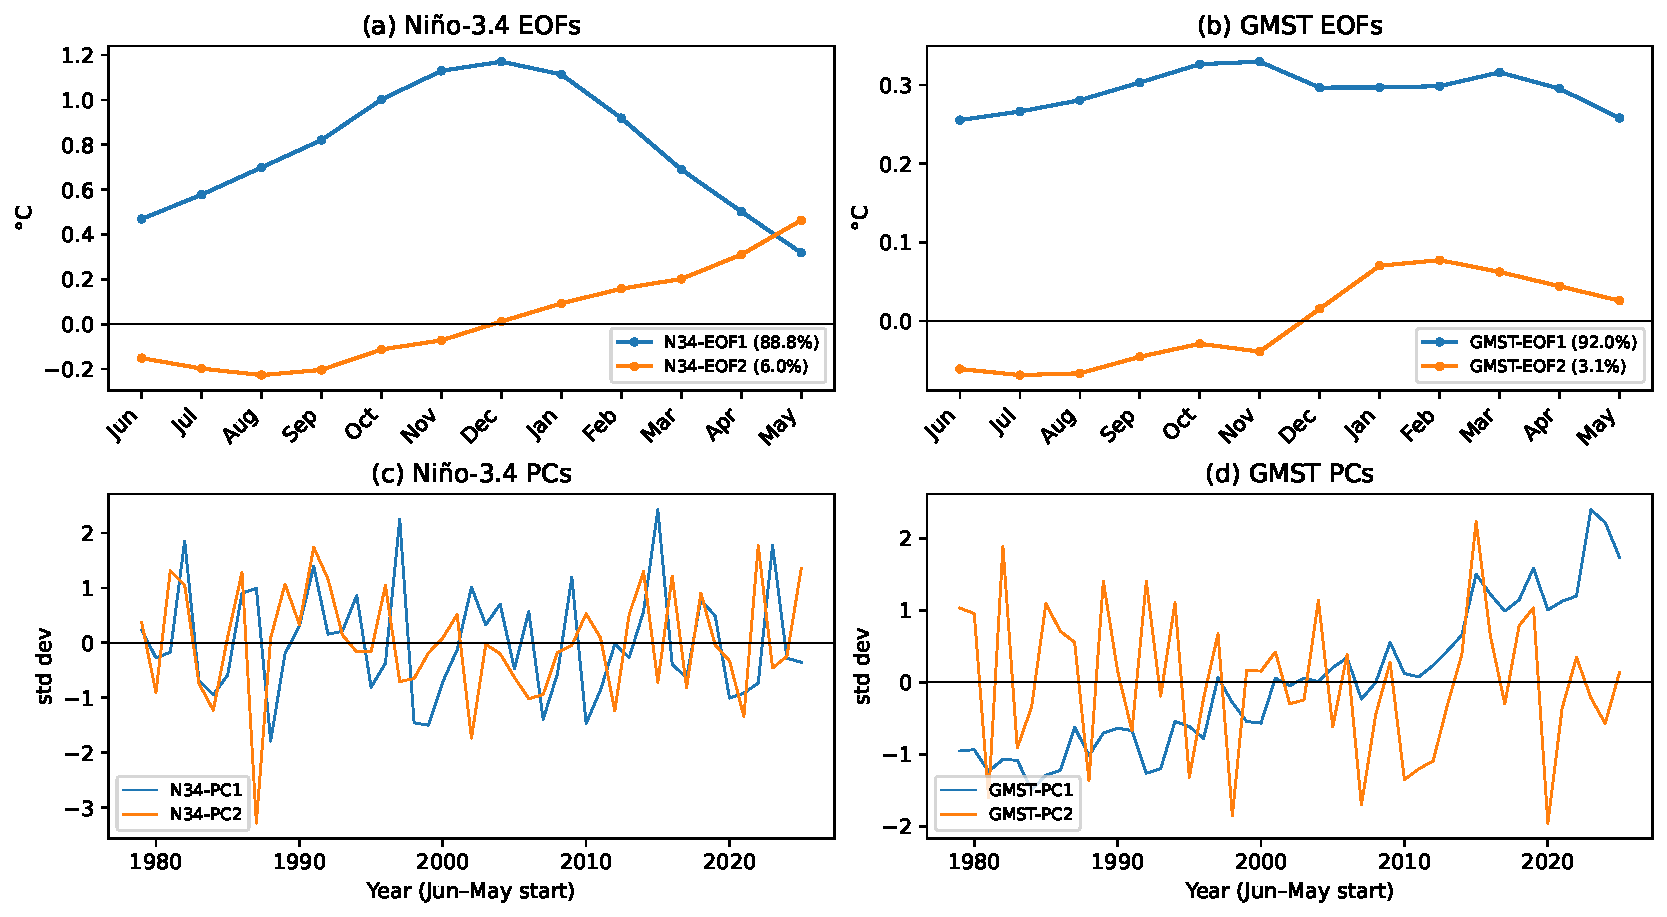
\includegraphics[width=\textwidth]{../figures/eofs_pcs.pdf}
  \noindent 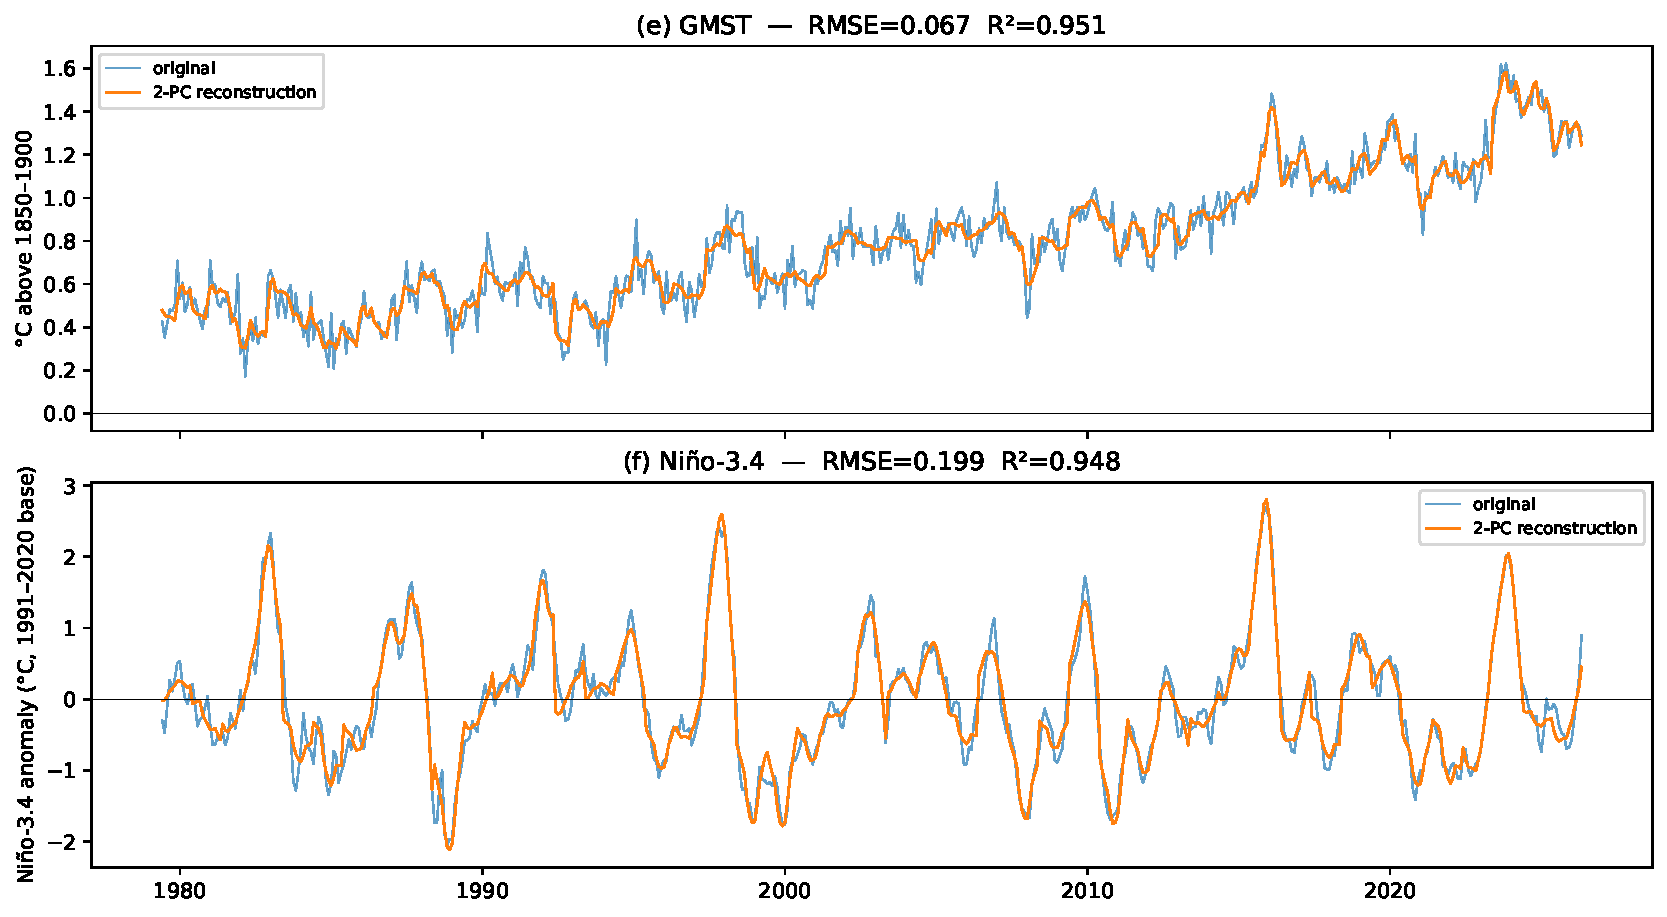
\includegraphics[width=\textwidth]{../figures/reconstruction_2pc.pdf}
  \caption{The leading two EOFs of June--May trajectories
      of (a) Ni\~no-3.4 and (b) global mean surface temperature
      (GMST). The corresponding leading two PCs of (c) Ni\~no-3.4 and
      (d) GMST.  Two-PC reconstructions of (e) Ni\~no-3.4 and (f) GMST
      with root-mean-squared error (RMSE) and $R^2$ values in the
      title.}
  \label{fig:fig1}
\end{figure}

The regression model in (\ref{eq:full}) is high-dimensional with 24 predictors and 12 predictands. The matrices $\bm{A}_{12}$ and $\bm{B}_{12}$ together contain 288 coefficients. To avoid overfitting, facilitate interpretation, and reduce the complexity of the model, we applied PCA to the two datasets. PCA is an unsupervised and systematic dimension-reduction method that optimizes explained variance and, as used here, ignores relationships between predictors and predictands. Previous work found that 12-month Ni\~no-3.4 trajectories are well approximated by one or two PCs, both in observations and in seasonal forecasts \cite{Bunge2009verified,Tippett2019:ENSO}. Consistent with those results, we found that approximately 95\% of the variability of June--May Ni\~no-3.4 segments is explained by the first two PCs (Fig.\ \ref{fig:fig1}a). Moreover, the same is true of GMST---approximately 95\% of the variability of a June--May GMST trajectory is explained by the first two PCs (Fig.\ \ref{fig:fig1}b).

Although PCA need not yield physically meaningful or readily explainable components, the leading PCs of GMST and Ni\~no-3.4 trajectories admit relatively clear interpretations. EOF1 of Ni\~no-3.4 peaks in December, reflecting the seasonal phase locking of ENSO (Fig.\ \ref{fig:fig1}a).  EOF2 of Ni\~no-3.4 is a dipole in time centered on December. The dipole structure is related to the mathematical requirement that EOF2 be orthogonal to EOF1 and serves to represent features such as shifts of the Ni\~no-3.4 peak and ENSO events that persist longer or decay more rapidly. EOF1 of GMST is nearly uniform across months (Fig.\ \ref{fig:fig1}b) and its PC has a clear upward trend (Fig.\ \ref{fig:fig1}d); together they represent a nearly month-independent warming trend. EOF2 of GMST is negative and roughly uniform over the June--November period until it rises in December and peaks in January and February, while PC2 shows no visible trend. The asymmetry of the dipole structure of EOF2 suggests that it represents the delayed post-peak response of GMST to ENSO via the atmospheric bridge \cite{Alexander2002atmospheric,Klein1999remote}. Reconstructions of Ni\~no-3.4 and GMST show that two EOFs are adequate to capture interannual variability ($R^2$ values of about 95\%; Fig.\ \ref{fig:fig1}e, f), although more unresolved subannual variability is visible in the GMST time series than in the Ni\~no-3.4 time series because much of the GMST variance is associated with its long-term trend.

The PCA analysis motivates replacing (\ref{eq:full}) with the four-PC model: \begin{linenomath*}
\begin{equation} \begin{bmatrix} \text{GMST-PC1}\\ \text{GMST-PC2}\\ \end{bmatrix}(y+1) = \bm{A}_{\text{4-PC}} \begin{bmatrix} \text{GMST-PC1}\\ \text{GMST-PC2}\\ \end{bmatrix}(y) + \bm{B}_{\text{4-PC}} \begin{bmatrix} \text{N34-PC1}\\ \text{N34-PC2}\\ \end{bmatrix} (y+1)\,, \label{eq:pc4} \end{equation}
\end{linenomath*} where the $2 \times 2$ matrices $\bm{A}_{\text{4-PC}}$ and $\bm{B}_{\text{4-PC}}$ represent, respectively, the dependence of the first two PCs of GMST on their prior values and on the contemporaneous values of PC1 and PC2 of Ni\~no-3.4. The number of coefficients is now reduced from 288 to eight.

\begin{figure}
  \noindent 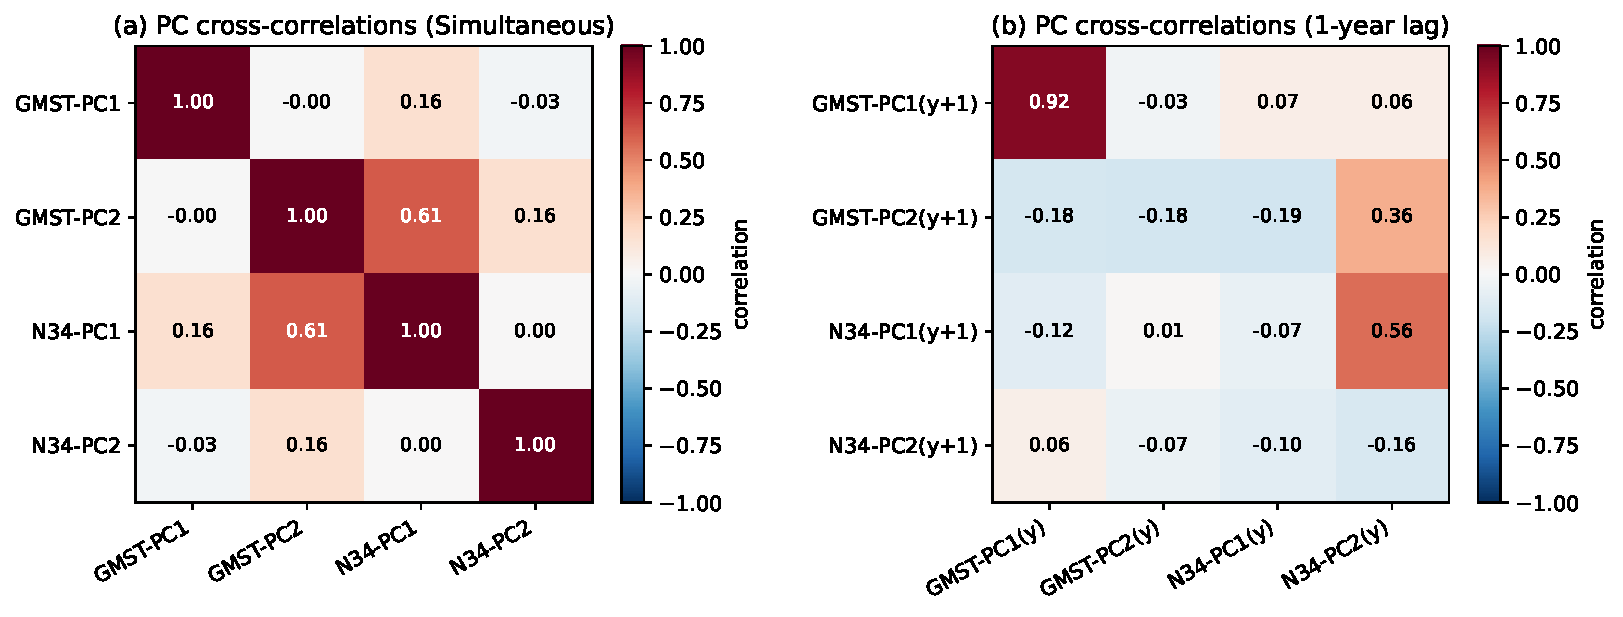
\includegraphics[width=\textwidth]{../figures/pc_correlations.pdf}
  \noindent 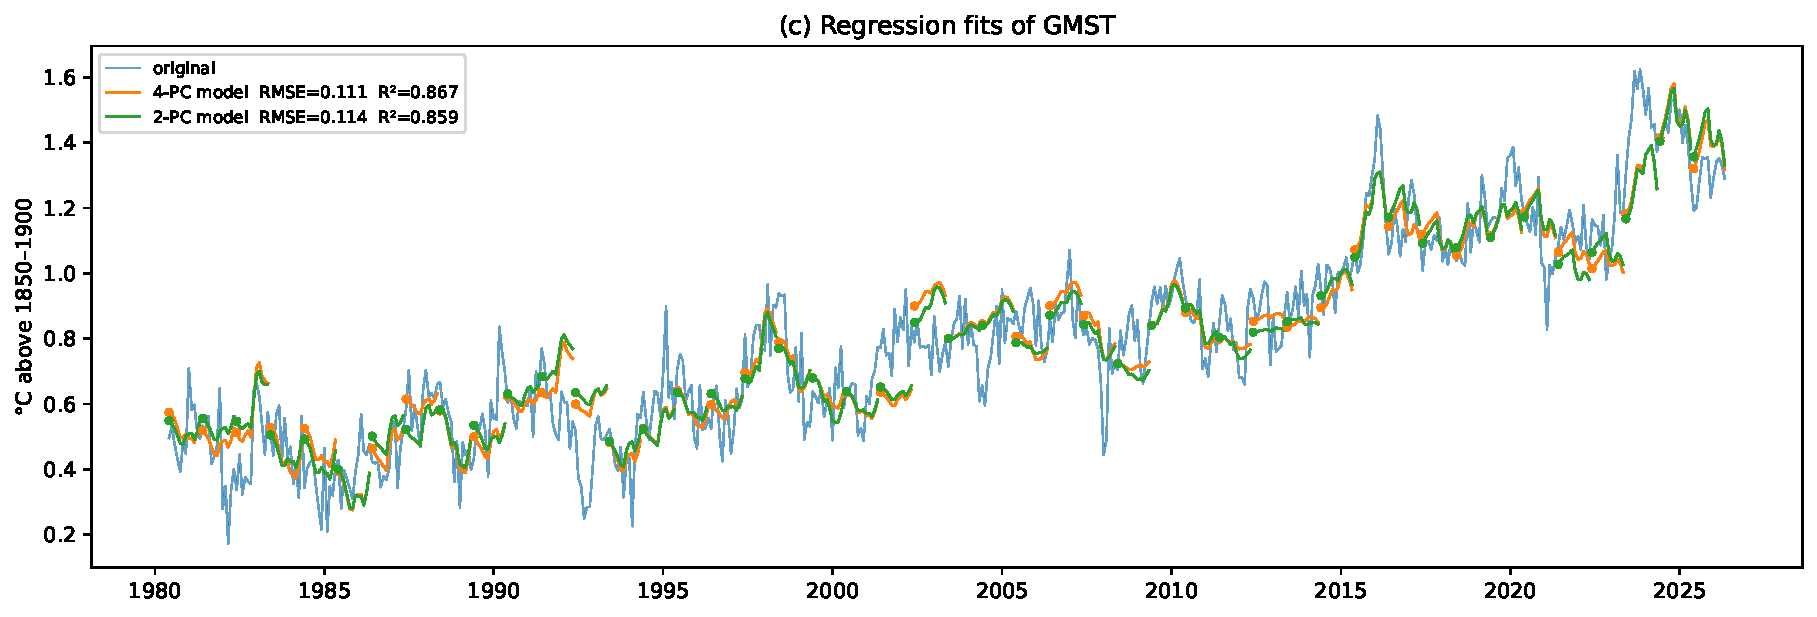
\includegraphics[width=\textwidth]{../figures/fit_all.pdf}
  \caption{(a) Simultaneous and (b) one-year lag correlations between
    the first two PCs of Ni\~no-3.4 and global mean surface
    temperature (GMST).  Panel (c) shows the GMST time series and its
    fit by the four-PC and two-PC models (see text for model
    details). Dots indicate June--May segment starts. Model RMSE and
    $R^2$ are shown in the legend.}
  \label{fig:fig2}
\end{figure}

We next examined the simultaneous and lagged correlations of the first two PCs of Ni\~no-3.4 and GMST. The strongest simultaneous correlation is the 0.61 correlation between N34-PC1 and GMST-PC2, which supports our hypothesis that GMST-EOF2 represents the delayed GMST response to ENSO (Fig. \ref{fig:fig2}a). The other simultaneous correlations are weak ($R^2 < 4\%$). The strongest lagged relation between PCs is the 0.92 correlation between GMST-PC1$(y)$ and GMST-PC1$(y+1)$, which reflects the upward trend in GMST-PC1 and the resulting strong year-to-year persistence (Fig. \ref{fig:fig2}b).  In contrast, the lag-1 autocorrelation of GMST-PC2 is small and negative ($r=-0.18$), consistent with the interpretation of GMST-PC2 as an ENSO response with little persistence from one year to the next. The source of the correlation between N34-PC2$(y)$ and N34-PC1$(y+1)$ is less clear, though it is visually evident in the PC time series (Fig.\ \ref{fig:fig1}c). It might reflect imperfect alignment of the June--May year with the ENSO life cycle. The correlation between N34-PC2$(y)$ and GMST-PC2$(y+1)$ ($r=0.36$) is explained almost entirely by the pathway N34-PC2$(y) \rightarrow$ N34-PC1$(y+1) \rightarrow$ GMST-PC2$(y+1)$. After accounting for N34-PC1$(y+1)$, the partial correlation between N34-PC2$(y)$ and GMST-PC2$(y+1)$ is only 0.03.

The correlation analysis above suggests that little is lost by using only two PCs as predictors: GMST-PC1$(y)$ and N34-PC1$(y+1)$. The two-PC model is: \begin{linenomath*}
\begin{equation} \begin{bmatrix} \text{GMST-PC1}\\ \text{GMST-PC2}\\ \end{bmatrix}(y+1) = \bm{A}_{\text{2-PC}} \; \text{GMST-PC1} (y) + \bm{B}_{\text{2-PC}} \; \text{N34-PC1} (y+1)\,, \label{eq:pc2} \end{equation}
\end{linenomath*} where the $2 \times 1$ matrices $\bm{A}_{\text{2-PC}}$ and $\bm{B}_{\text{2-PC}}$ represent, respectively, the dependence of the first two PCs of GMST on the prior value of PC1 of GMST and on the contemporaneous value of PC1 of Ni\~no-3.4. The number of coefficients is reduced from eight to four. The fit obtained with these two predictors is nearly identical to that obtained with four predictors (Fig.\ \ref{fig:fig2}c), consistent with only the coefficients of GMST-PC1$(y)$ and N34-PC1$(y+1)$ being large and statistically significant in the four-predictor model (Table \ref{tab:full_model}) and their having nearly the same values in the two-predictor model (Table \ref{tab:model-r1}).

While the two-PC predictor model is effective and parsimonious, further simplifications can improve interpretability. In particular, the predictors GMST-PC1$(y)$ and N34-PC1$(y+1)$ are defined by the PCA itself and depend on the specific data used. Replacing the predictor PCs with quantities that closely approximate them, but whose calculation is more transparent, would yield a more explainable model. Because N34-PC1 is highly correlated ($r>0.98$) with the December Ni\~no-3.4 value (Fig.\ \ref{fig:fig3}a), we replaced N34-PC1 with December Ni\~no-3.4. This close correspondence follows from the structure of the leading EOFs: EOF1 peaks in December, while EOF2 is close to zero in December. We replaced GMST-PC1 with the June--May mean GMST, which we refer to as the GMST level. The GMST level is highly correlated with GMST-PC1 ($r>0.99$; Fig.\ \ref{fig:fig3}b) because GMST-EOF1 is nearly uniform across months. This replacement suggests an alternative decomposition of GMST in which the first component is simply the level (June--May mean), and the second component captures as much as possible of the remaining variance. We implemented this idea by decomposing each June--May GMST trajectory into its June--May level and departures from that level, and then applying PCA to the departures. Because this decomposition removes both monthly means and June--May means, we call it double-centered PCA (DC-PCA). Although DC-PCA is not variance-optimal, the loss is small: the variance explained by the first two modes decreases from 95.1\% to 94.6\% (Fig.\ \ref{fig:EOF-variance-explained-dc}). The leading EOF from the double-centered decomposition is similar to GMST-EOF2 (Fig.\ \ref{fig:fig3}b), and GMST-DC-PC1 is also similar to GMST-PC2, with correlation 0.992 (Fig.\ \ref{fig:fig3}b).

These replacements (N34-PC1 replaced by December Ni\~no-3.4 and GMST-PC1 replaced by level) give the simplified model: \begin{linenomath*}
\begin{equation} \begin{bmatrix} \text{GMST}_{\text{level}}\\ \text{GMST-DC-PC1}\\ \end{bmatrix}(y+1) = \bm{A} \; \text{GMST}_{\text{level}} (y) + \bm{B} \; \text{Ni\~no-3.4}_{\text{Dec}} (y+1)\,, \label{eq:simplified} \end{equation}
\end{linenomath*} where the $2 \times 1$ matrices $\bm{A}$ and $\bm{B}$ represent, respectively, the dependence of the GMST level and GMST-DC-PC1 on the prior value of the GMST level and on the contemporaneous December value of Ni\~no-3.4 (regression summary in Table \ref{tab:model-sm}). The performance of the simplified model is nearly identical to that of the two-PC predictor model (Fig.\ \ref{fig:fig3}c).

An attractive feature of the simplified model is that, once the recent GMST level is specified, the shape of the predicted GMST response is fixed and only its amplitude changes with the December Ni\~no-3.4 value. Figure \ref{fig:fig3}d shows the implied June--May GMST response per $+1$\textdegree C of December Ni\~no-3.4. The response is about $0.03$\textdegree C during June--August, rises sharply beginning in December, and peaks at about $0.11$\textdegree C in February. The same analysis using relative Ni\~no-3.4 gives a similar GMST response (Fig.\ \ref{fig:fig3}d), indicating that the result is not sensitive to the choice of ENSO index. The slightly weaker response obtained with relative Ni\~no-3.4 reflects its larger December variance during this period---about 8\% greater than that of the traditional Ni\~no-3.4 index---rather than weaker correlation with GMST residuals (Fig.\ \ref{fig:corr_res}; Table \ref{tab:model-sm-roni}). The simplified model allows statements of the form: ``given the recent 12-month average of GMST and the expected December Ni\~no-3.4 value, the June--May GMST trajectory is expected to be \ldots''. Specifically, the observed June 2025--May 2026 GMST level of 1.3\textdegree C and an NMME-forecast December 2026 Ni\~no-3.4 value of $+3.3$\textdegree C gives a predicted February 2027 peak near 1.6\textdegree C above preindustrial (Fig.\ \ref{fig:fig3}e). For comparison, we show the NMME GMST forecast (June 2026 initialization) whose values peak near 1.8\textdegree C.

\begin{figure}
  \noindent 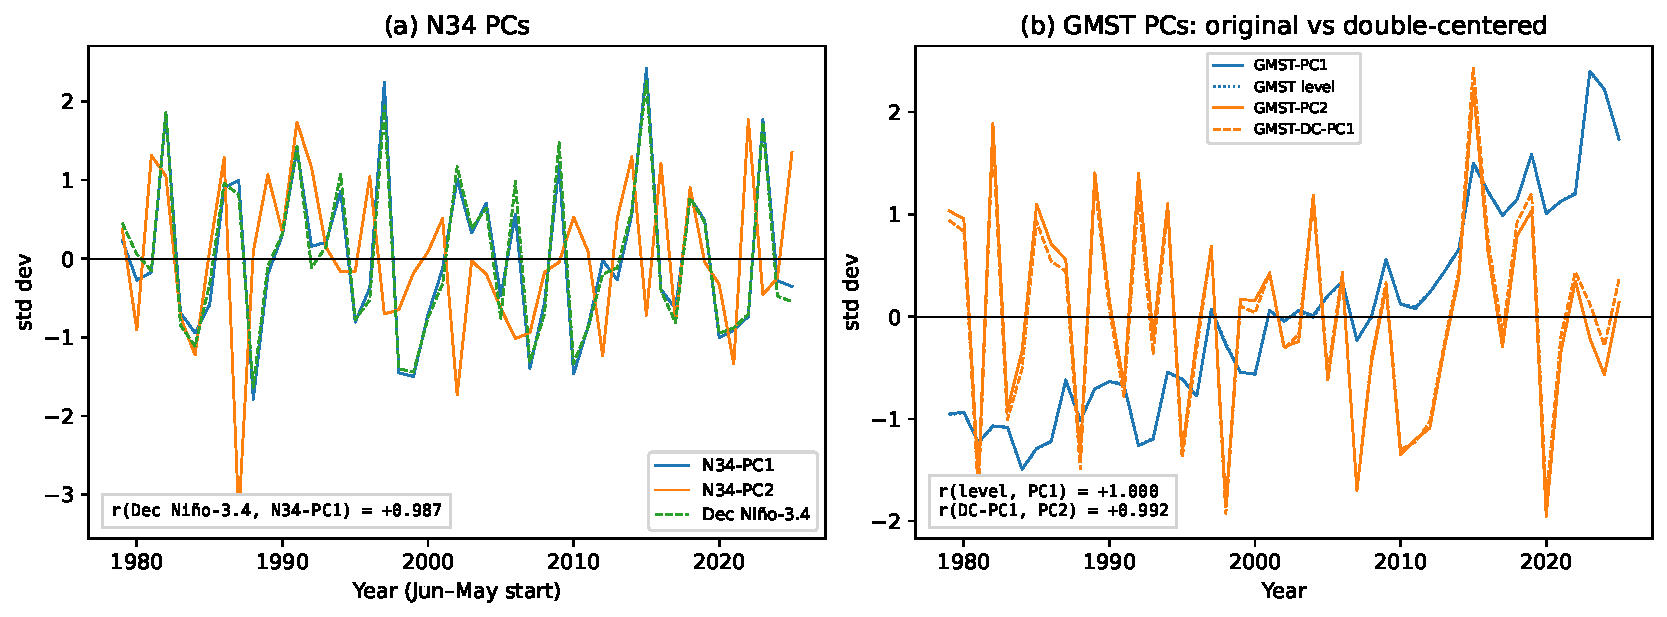
\includegraphics[width=\textwidth]{../figures/simplified_pred.pdf}
  \noindent 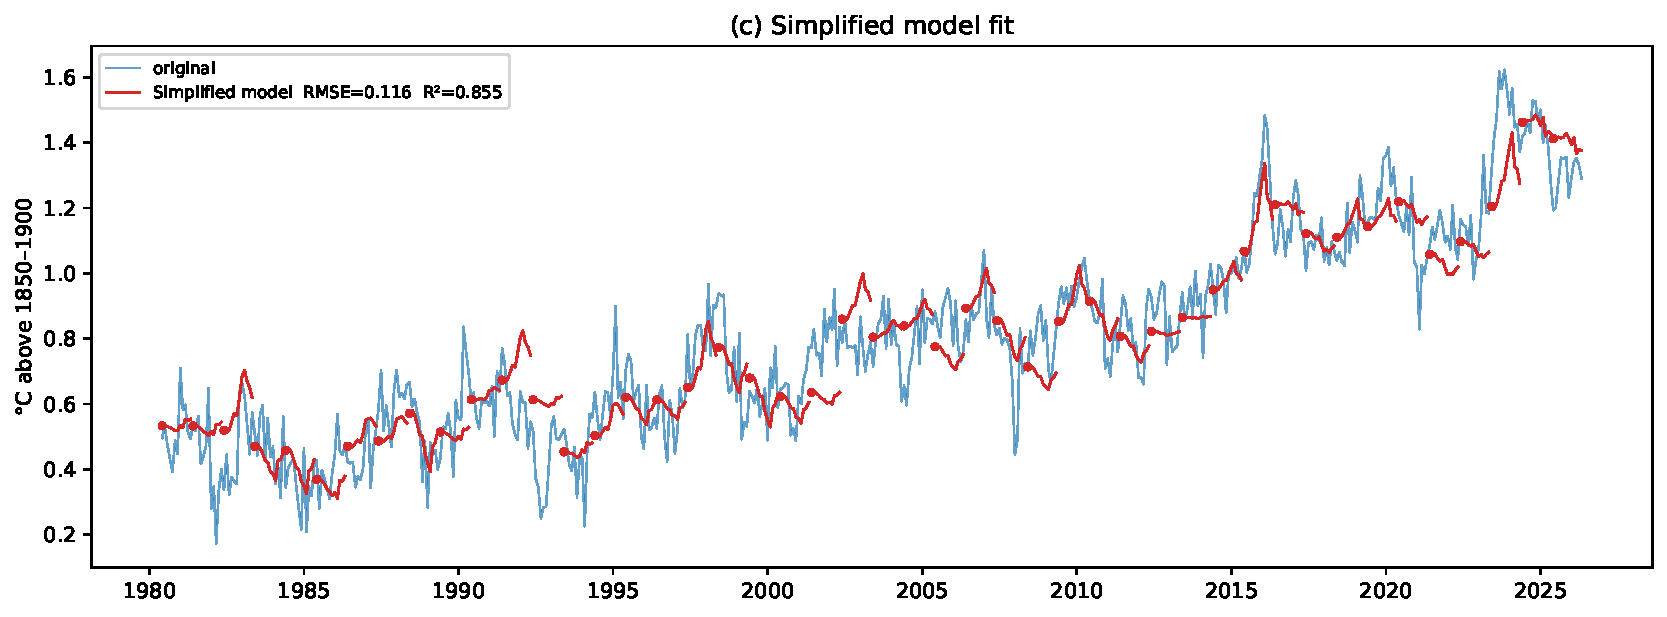
\includegraphics[width=\textwidth]{../figures/fit_idea2.pdf}
  \noindent 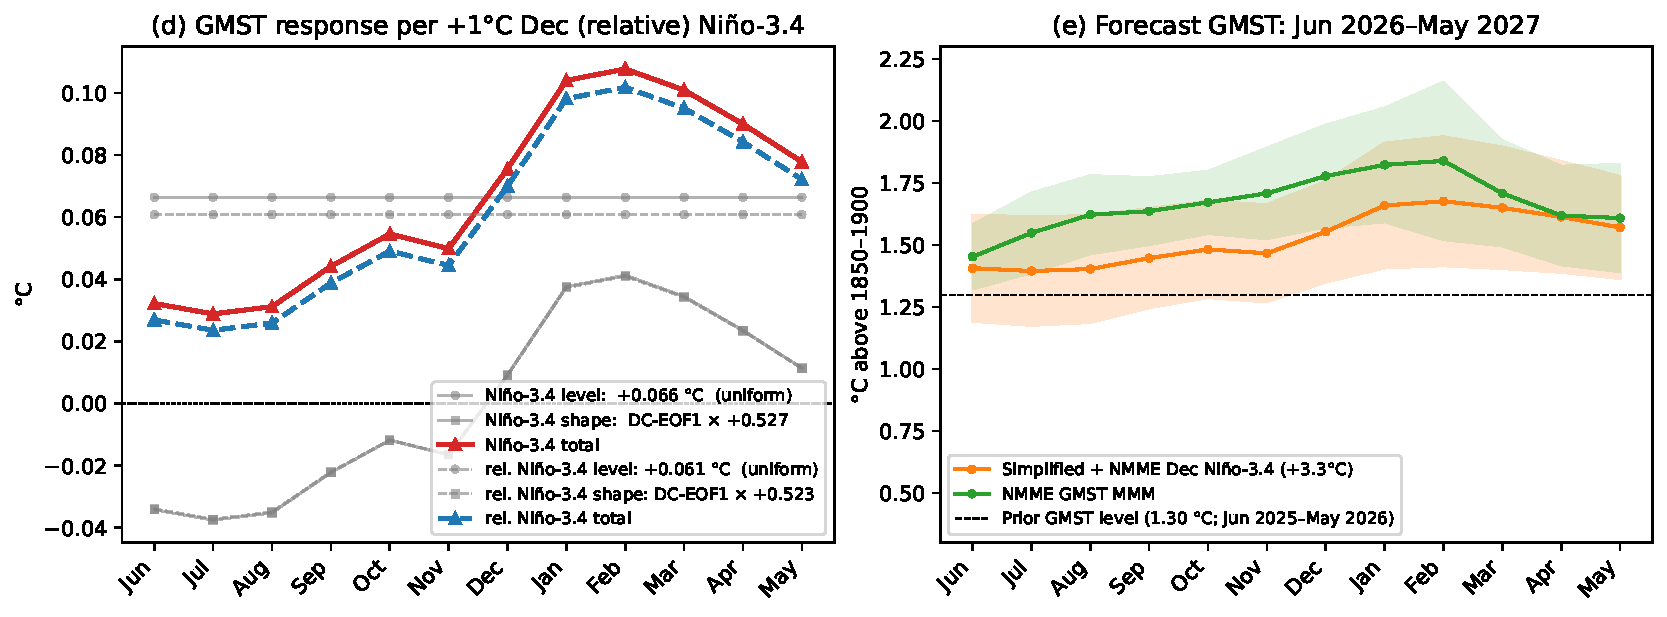
\includegraphics[width=\textwidth]{../figures/forecast.pdf}
  \caption{Comparisons of (a) N34-PC1 with December Ni\~no-3.4 and (b)
    GMST PCs with GMST level and GMST-DC-PC1. Panel (c) shows the GMST
    time series and its fit by the simplified model (see text for
    details). Panel (d) shows the implied June--May GMST response per
    $+1$\textdegree C of December Ni\~no-3.4 and relative
    Ni\~no-3.4. Panel (e) shows NMME ($\pm$2 std shading) and
    simplified model (95\% prediction interval) forecasts of June
    2026--May 2027 GMST}
  \label{fig:fig3}
\end{figure}

Having derived the simplified regression model, we next addressed three important questions: \begin{itemize} \item How much is gained by accounting for ENSO?  \item How much does performance change when forecast rather than observed December Ni\~no-3.4 is used?  \item How does the simplified regression model compare with initialized climate forecasts of GMST? \end{itemize} This comparison helps to determine whether the simplified statistical model captures information already represented in dynamical forecasts, or whether the dynamical forecasts provide additional predictive information. To address the first question, we considered two persistence-only benchmarks: one based on the preceding June--May mean GMST and one based on the preceding May GMST value. To address the second and third questions, we used NMME multi-model-mean forecasts of December Ni\~no-3.4 and monthly GMST.

To compare the simplified regression model with the NMME forecasts, we looked at trends and the relation in the models of December Ni\~no-3.4 with GMST level and GMST-DC-PC1. The NMME models broadly reproduce the observed ENSO--GMST relationships, although with notable model differences (Fig.\ \ref{fig:nmme_dc_pca}; Table \ref{tab:trends}). Several models have GMST trends that are significantly larger than observed, as noted previously \cite{Delsole2025diagnosing,Swart2019canadian,Tippett2024trends}. For the correlation between GMST level and December Ni\~no-3.4, CanESM5 and GEM5.2-NEMO are stronger than observed (Fig.\ \ref{fig:nmme_dc_pca}).  These two models also have the most positive December Ni\~no-3.4 trends (Table \ref{tab:trends}). The COLA-RSMAS-CCSM4 GMST-Ni\~no-3.4 correlation is weaker than observed, while the remaining models are close to observations. For the relation between GMST-DC-PC1 and December Ni\~no-3.4, COLA-RSMAS-CCSM4 is again much weaker than observed ($r=0.20$ compared with $r=0.62$). The remaining model correlations are slightly weaker than observed, with the exception of NCEP-CFSv2.

We next assessed performance relative to the persistence-only benchmarks. Both the simplified regression model and the NMME forecasts outperform the prior June--May mean benchmark in every month, as measured by RMSE (Fig.\ \ref{fig:fig4}a). The May-value benchmark is more competitive early in the June--May year, particularly in June and July. Compared with this benchmark, both the simplified model and the NMME forecasts have lower RMSE from August through May. For the simplified regression model, there is little difference between using observed December Ni\~no-3.4 and using forecast December Ni\~no-3.4, and the RMSE differences are statistically insignificant in most months (Table \ref{tab:rmse-sig}). The NMME forecasts of GMST have lower RMSE than the simplified model for target months June through December, and similar RMSE for later target months. The largest NMME advantage occurs in October, and the RMSE difference between the NMME GMST forecast and the simplified model using forecast December Ni\~no-3.4 is statistically significant (Table \ref{tab:rmse-sig}). We computed MSESS using the prior June--May GMST average as the reference forecast (Fig.\ \ref{fig:fig4}b). The resulting scores show that the simplified model improves most on persistence after December, consistent with the delayed GMST response to ENSO. In contrast, the NMME GMST forecasts show their largest advantage over persistence before December, especially in September and October. Results with leave-one-year-out cross validation and persistence plus trend baselines are similar (not shown).

Representative years illustrate these differences (Figs.\ \ref{fig:fig4}c--h). In cool ENSO years, the simplified model captures the winter cooling and spring rebound but with reduced amplitude, as expected from regression shrinkage. In warm ENSO years, it captures delayed warming, while the NMME forecasts are often closer to the observed level, especially in 2015--16 and 2023--24. The 2023--24 case warrants particular attention. First, it was at least partly predictable because the NMME captures much of the observed warming. Second, the role of El Ni\~no is unclear since the ENSO-based forecast fails to reproduce the June--November observed anomaly amplitude, and the September warming is not at the typical time when ENSO signals appear \cite{Raghuraman20242023,Rantanen2024jump}.
\begin{figure}
  \noindent 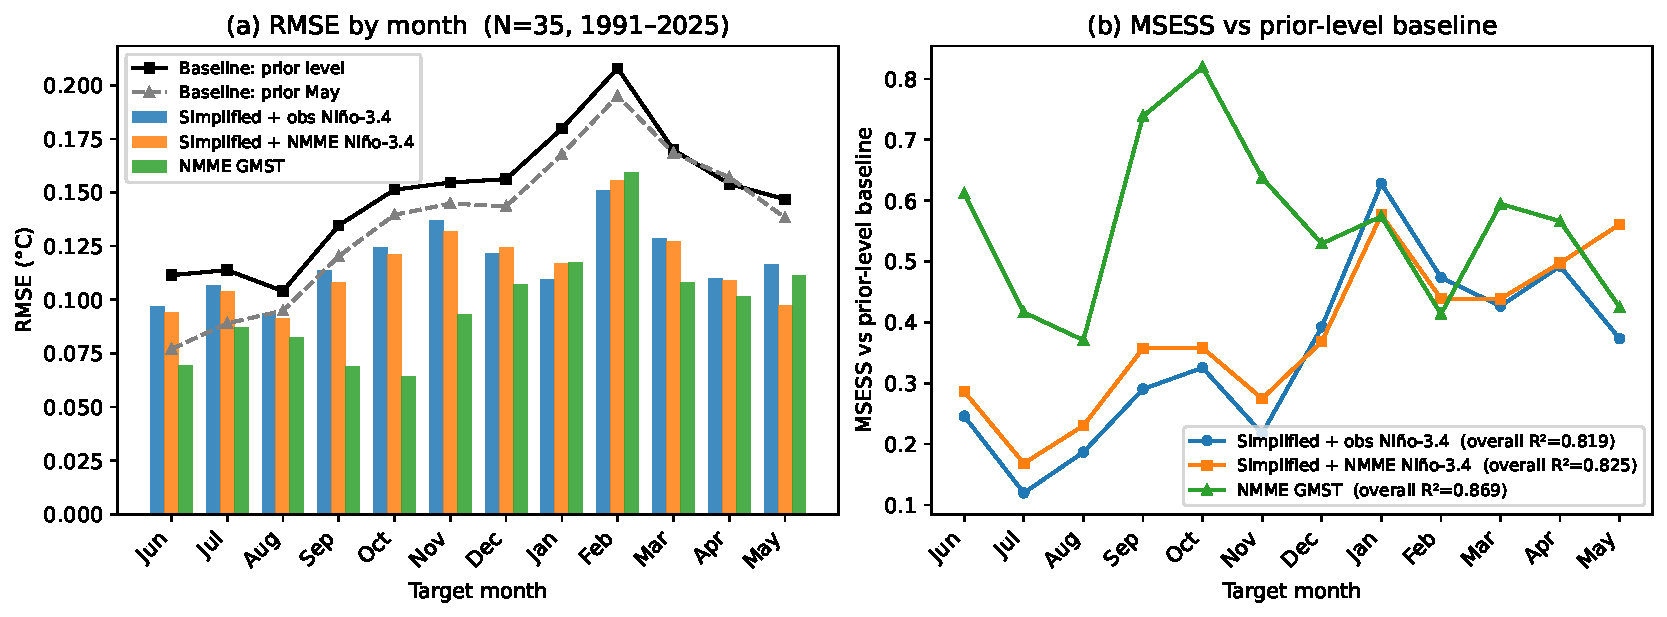
\includegraphics[width=\textwidth]{../figures/nmme_skill_comparison.pdf}
  \noindent 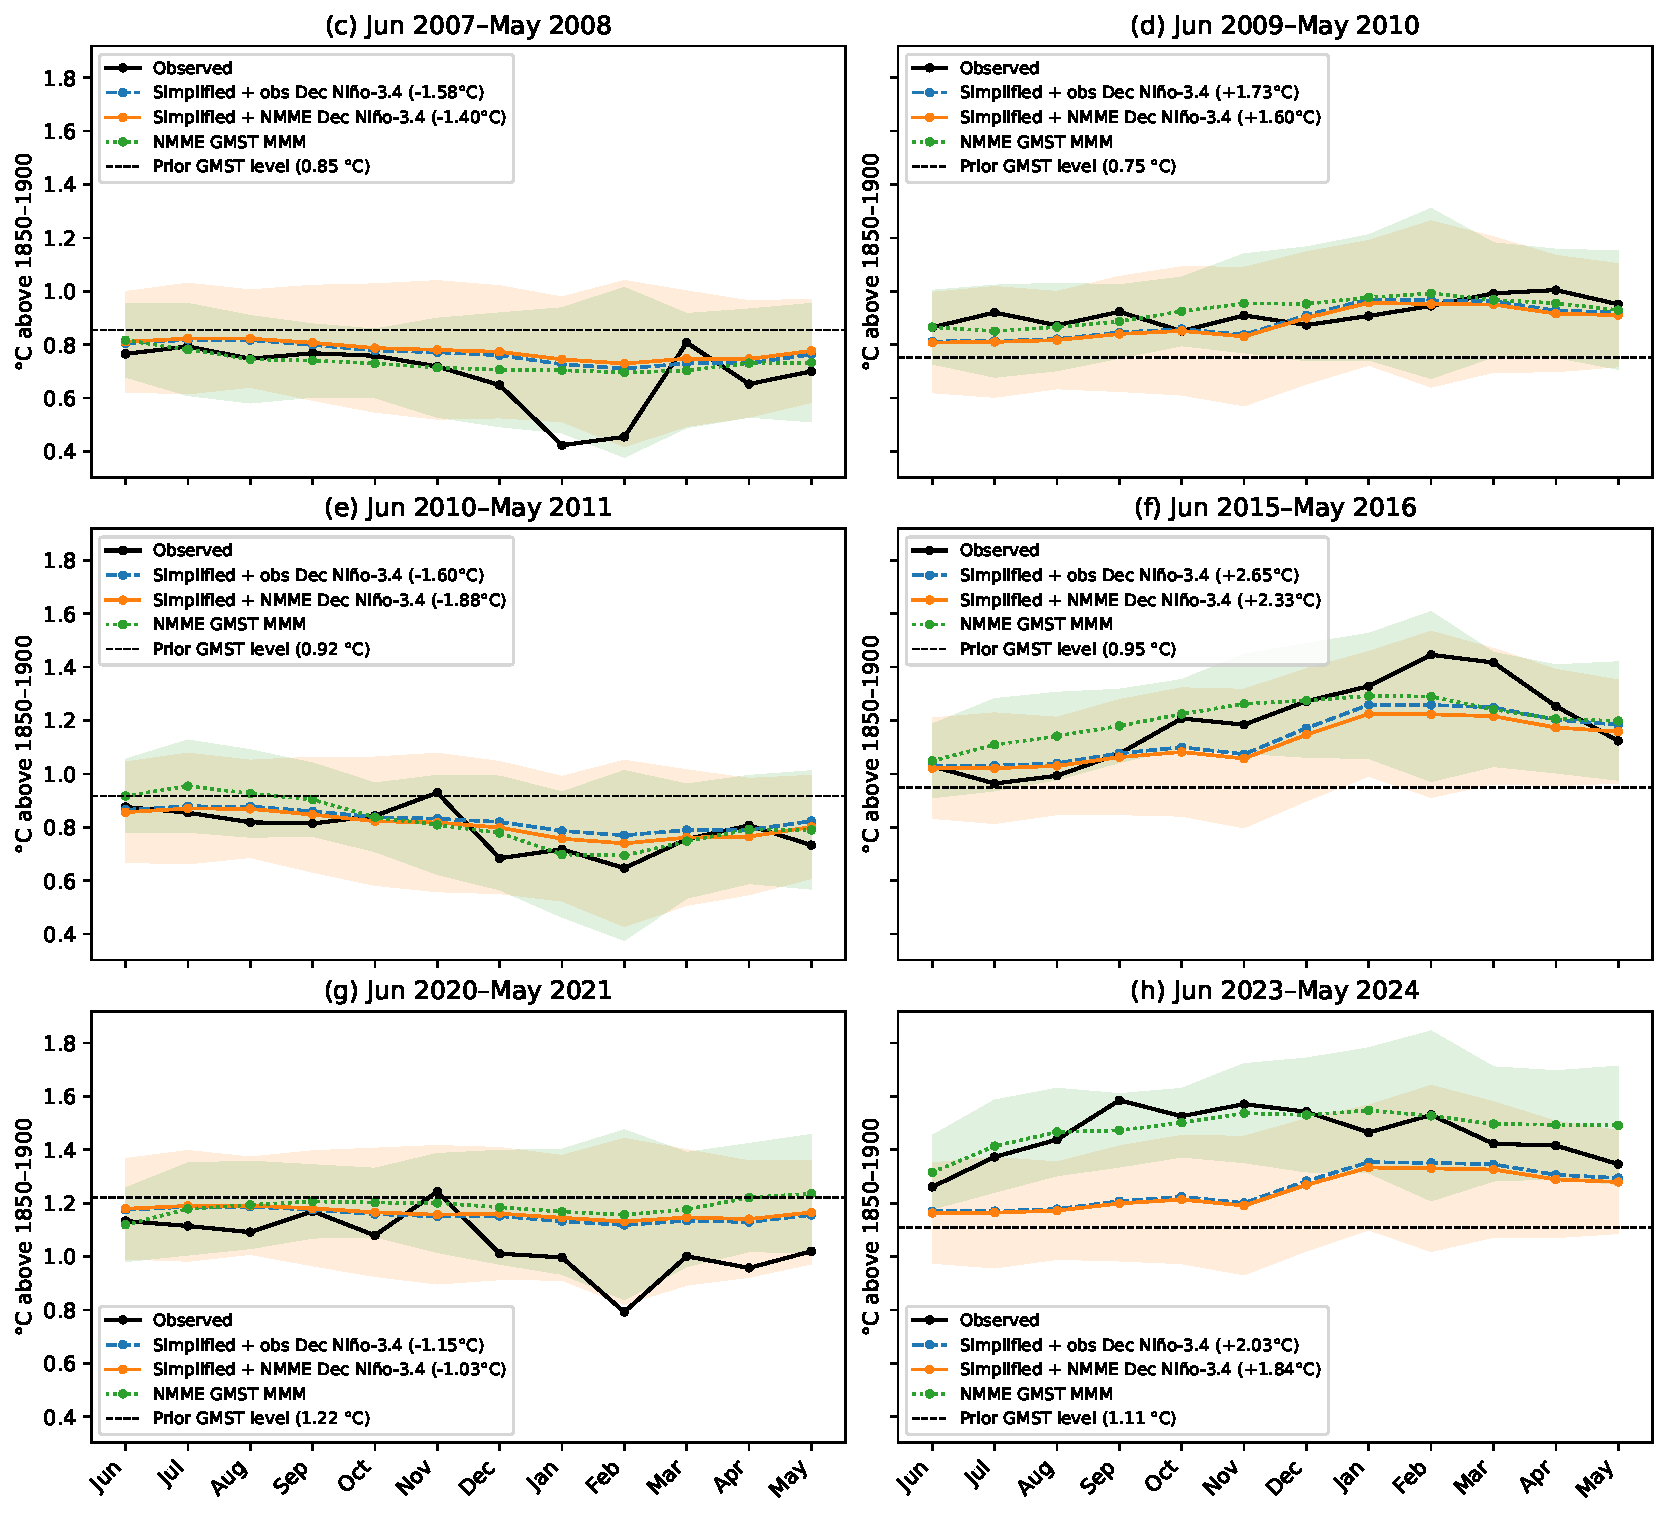
\includegraphics[width=\textwidth]{../figures/nmme_trajectory_examples.pdf}
  \caption{(a) Root-mean-squared error (RMSE) of the persistence
    baselines, the simplified model (using observed and forecast
    December Ni\~no-3.4), and NMME forecasts of June--May global mean
    surface temperature (GMST) 1991--2025.  (b) Mean-squared-error
    skill score (MSESS) of the simplified model and NMME forecasts
    relative to the prior June--May GMST level persistence baseline.
    Observed June--May GMST, simple model fits, and NMME GMST
    forecasts for (c) 2007--08, (d) 2009--10, (e) 2010--11, (f)
    2015--16, (g) 2020--21, and (h) 2023--24. The simplified model
    inputs: observed and NMME-forecast Ni\~no-3.4 values and prior
    GMST level are given in parenthesis. Shading as in Fig.\
    \ref{fig:fig3}e.}
  \label{fig:fig4}
\end{figure}

\section{Summary and discussion}\label{sec:summary}

Here we developed a simple and interpretable regression model that quantifies the relationship between ENSO and global mean surface temperature (GMST). The model allows the June--May evolution of monthly GMST to be anticipated based on information that is available near the beginning of June. We began with a high-dimensional formulation and applied a sequence of systematic, physically motivated simplifications to obtain a model with two predictors. The resulting predictors---recent GMST level and expected December Ni\~no-3.4 value---serve to model the persistence of GMST and its delayed response to ENSO. Principal component analysis (PCA) of 12-month June--May trajectories of GMST and Ni\~no-3.4 was especially useful because the first two PCs of GMST and Ni\~no-3.4 explain more than 95\% of the variance of June--May trajectories. The efficiency of PCA in explaining GMST evolution might be expected because a substantial fraction of GMST variance is associated with the long-term trend.  The result is more striking for Ni\~no-3.4 evolution, since a common view is that each ENSO event has its own distinct temporal structure.

The structure of the leading EOFs suggested further simplifications to improve interpretability. Since the leading EOF of GMST is nearly uniform across months, GMST-PC1 was replaced by the June--May average of GMST. The leading Ni\~no-3.4 EOF represents the typical temporal evolution of ENSO and peaks in December, so the corresponding PC was replaced by the December value of Ni\~no-3.4. These changes simplified the predictors with little loss of accuracy. According to the model, an expected December Ni\~no-3.4 anomaly of 1\textdegree C is associated with a GMST increase of about 0.03\textdegree C during June--August and a peak increase of about 0.11\textdegree C in the following February.

Although the ENSO contribution to GMST is modest, including ENSO improves prediction relative to persistence-only benchmarks. The simplified model reduces RMSE relative to the prior June--May mean benchmark in every month and relative to the prior May benchmark from August through May. The MSESS results show that this improvement is largest after December, consistent with the delayed GMST response to ENSO. Replacing observed December Ni\~no-3.4 with forecast December Ni\~no-3.4 produces little change in RMSE. By contrast, direct NMME forecasts of GMST show their largest advantage earlier in the June--May year, especially before December.

A broader implication is that ENSO information is most useful for GMST prediction when the forecast target is aligned with the ENSO life cycle. Calendar-year and annual-to-decadal forecast systems are valuable, but their initialization and verification windows are not optimized for taking advantage of post-spring-barrier ENSO predictability to anticipate June--May GMST evolution \cite{Hermanson2022wmo,WMO2025GADCU, Dunstone2024will,Folland2025review}. Initialized seasonal forecast systems, because they are run monthly, are better positioned to exploit the ENSO signal as it emerges and becomes reliable, although they still have known trend and ensemble-calibration errors \cite{LHeureux2022-Trends1,Mayer2025tropical,Tippett2024trends}. Despite these limitations, the NMME multimodel mean provides a useful benchmark here and added skill relative to the simplified regression model during the early part of the June--May forecast year.

\clearpage

%TC:ignore

\section*{Open Research Section}
NOAAGlobalTemp version 6.1 data are available from
% from
% \url{https://www.ncei.noaa.gov/data/noaa-global-surface-temperature/v6.1/access/gridded/NOAAGlobalTemp_v6.1.0_gridded_s185001_e202605_c20260608T115341.nc}
\citeA{NOAAGlobalTemp6p1}. NOAA Extended Reconstructed SST V5 (ERSSTv5) data are available from \citeA{NCEIERSSTv5}. % provided by the NOAA PSL, Boulder, Colorado, USA, from their website at \url{https://downloads.psl.noaa.gov/Datasets/noaa.ersst.v5/sst.mnmean.nc}.
Monthly values of the relative Ni\~no-3.4 index are available from \citeA{RONImonthly}. % \url{https://www.cpc.ncep.noaa.gov/data/indices/Rnino34.ascii.txt}.
  NMME data are available from \citeA{ENSO-conditioned-data}. % the IRI Data Library \url{https://iridl.ldeo.columbia.edu/SOURCES/.Models/.NMME/} and the Zenodo archive \url{https://doi.org/10.5281/zenodo.20514351}.

\section*{Conflict of Interest}
The authors declare no conflicts of interest.

\acknowledgments
We thank Michelle L. L\textquotesingle Heureux for helpful discussions and suggestions and two anonymous reviewers for their useful comments. Support from NSF is acknowledged by EJB (2223262). The authors also acknowledge the use of AI tools, including OpenAI's ChatGPT and Anthropic's Claude, to assist with code and manuscript editing.

\bibliography{references}
%% SI_BEGIN
\clearpage
\setcounter{page}{1}

\section*{Supporting Information for ``ENSO-conditioned evolution of global mean surface temperature''}
\begin{center}
\noindent
\authors{Michael K. Tippett$^1$ and Emily
  J. Becker$^2$}

\noindent $^1${Department of Applied Physics and Applied Mathematics, Columbia University, New York, New York}

\noindent $^2${Rosenstiel School of Marine, Atmospheric, and Earth Science, University of Miami, Miami, Florida}

\end{center}

\noindent\textbf{Contents of this file}
%%%Remove or add items as needed%%%
\begin{enumerate}
%\item Text S1 to Sx
\item Figures S1 to S3
\item Tables S1 to S6
%if Tables are larger than 1 page, upload as separate excel file
\end{enumerate}

\clearpage

\renewcommand\thefigure{S\arabic{figure}}

\setcounter{figure}{0}

\renewcommand\thetable{S\arabic{table}}

\setcounter{table}{0}

\begin{figure}
  \noindent 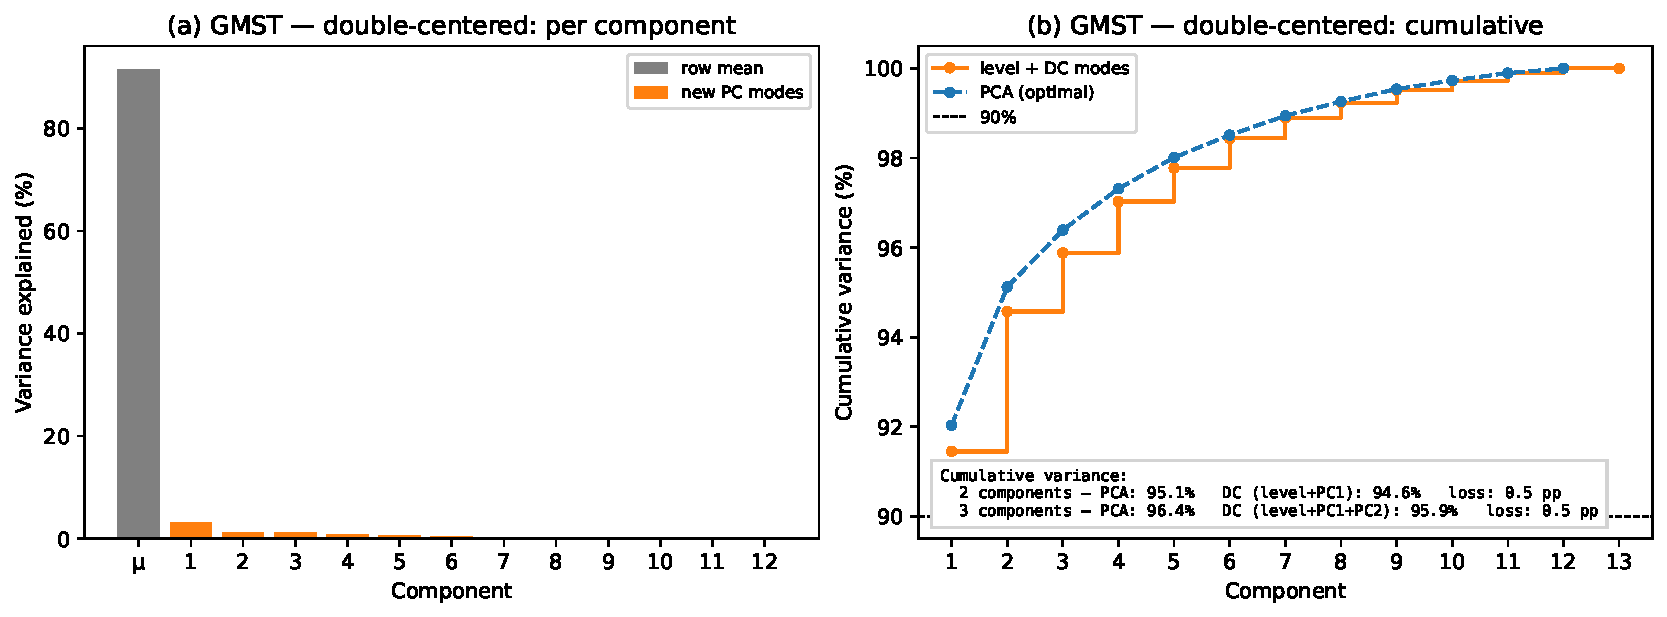
\includegraphics[width=\textwidth]{../figures/variance_explained_dc.pdf}
  \caption{Variance per mode and cumulative
      variance for GMST double-centered PCA.}
  \label{fig:EOF-variance-explained-dc}
\end{figure}

\begin{figure}
  \noindent 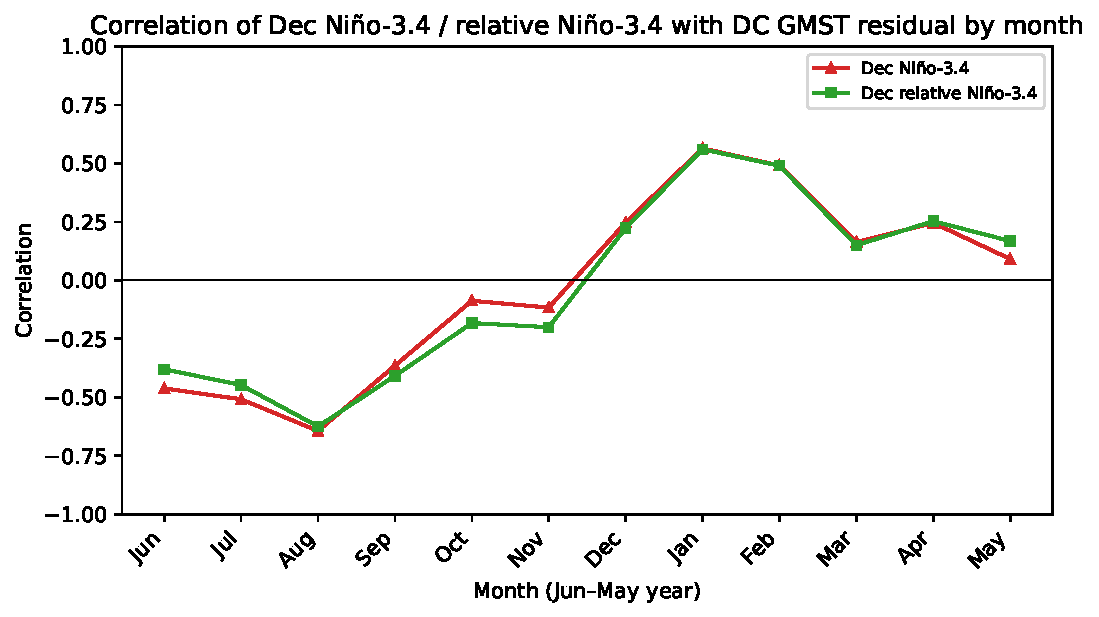
\includegraphics[width=\textwidth]{../figures/corr_dec_n34_by_month.pdf}
  \caption{December Ni\~no-3.4 and relative December
      Ni\~no-3.4 correlations with DC GMST residuals (level removed)
      by month.}
  \label{fig:corr_res}
\end{figure}

\begin{figure}
  \noindent 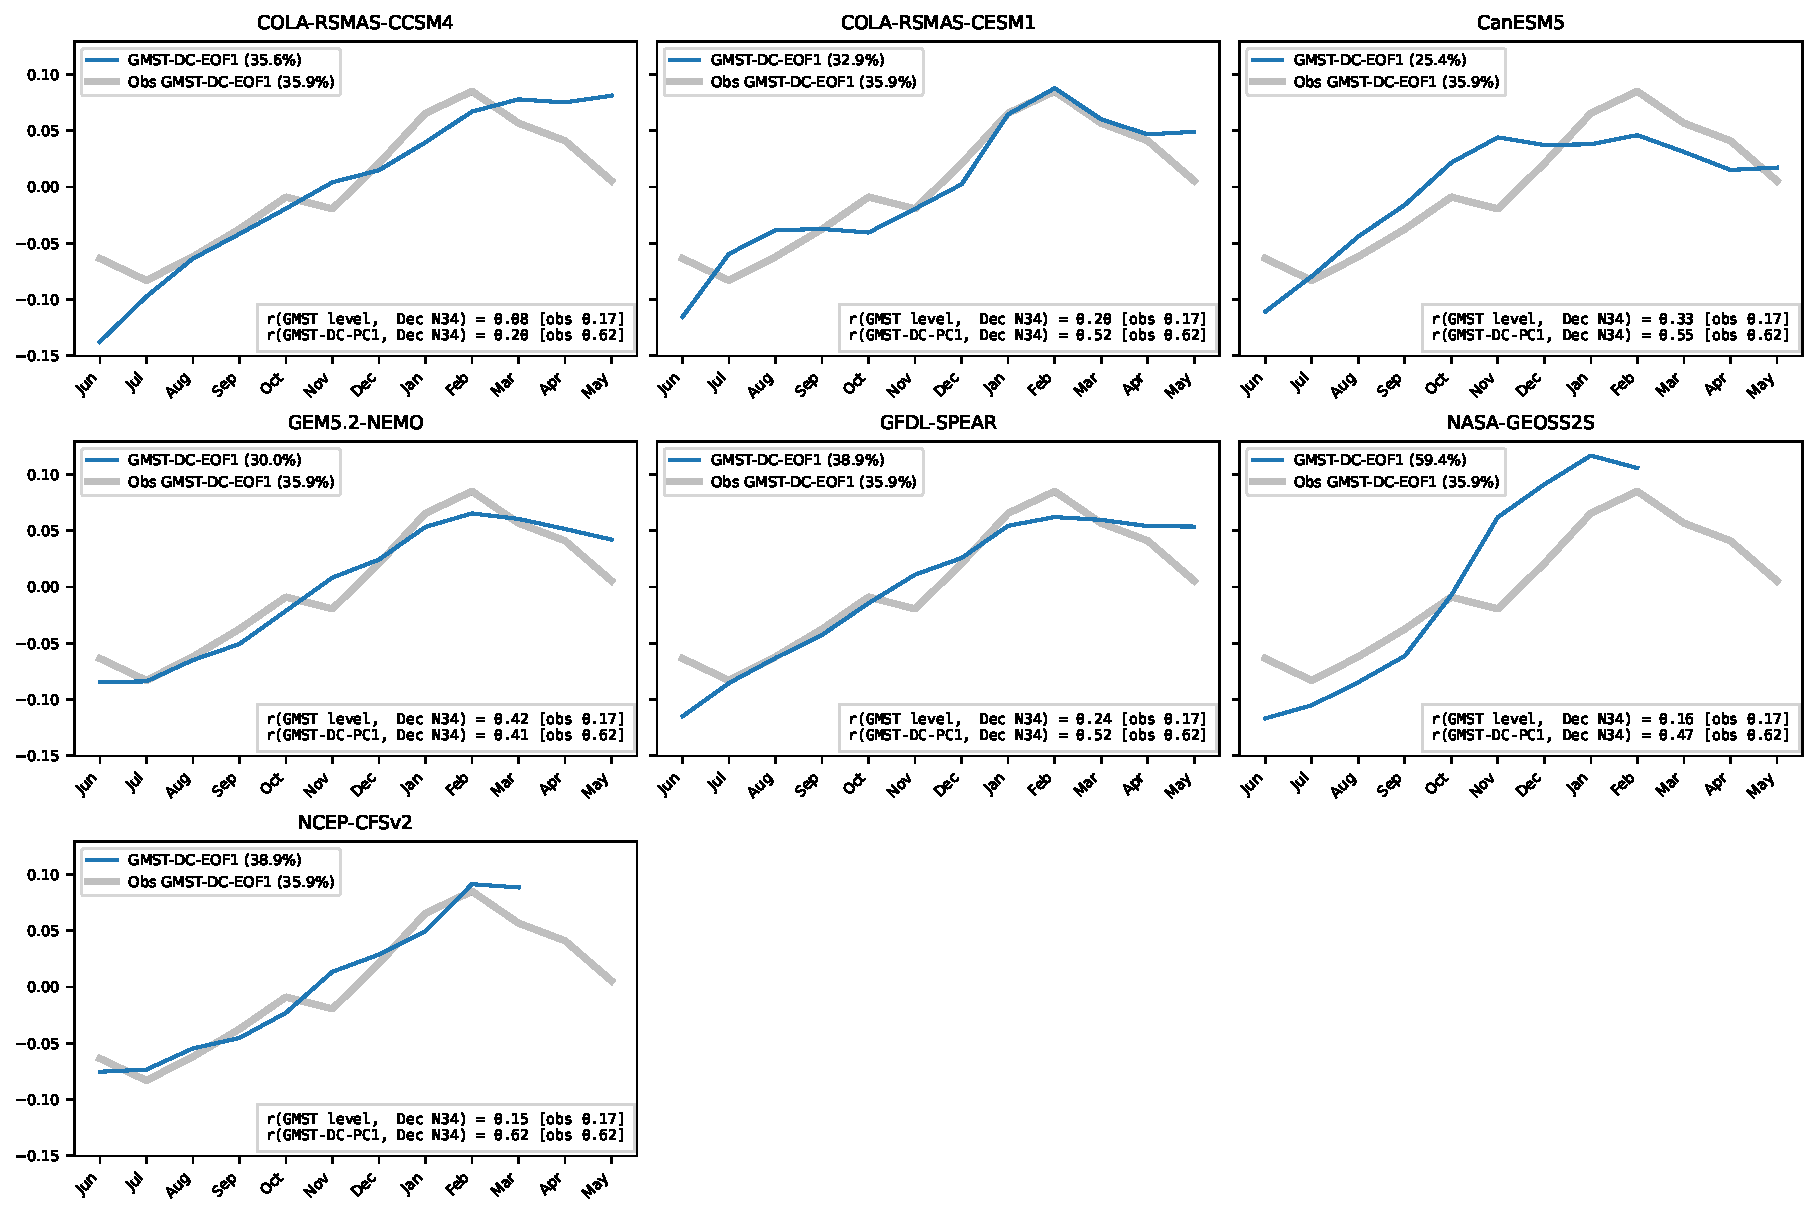
\includegraphics[width=\textwidth]{../figures/nmme_traj_dc_pca.pdf}
  \caption{The first double-centered EOF of GMST (GMST-DC-EOF1) in
    seven NMME models and observations. The text box shows the
    correlation of the model's Ni\~no-3.4 with the model's GMST level
    and DC-PC1. The observed values are in brackets for comparison.}
  \label{fig:nmme_dc_pca}
\end{figure}

\clearpage

\begin{table}
  \begin{tabular}{lll}
\hline
               & GMST-PC1$(t+1)$ & GMST-PC2$(t+1)$  \\
\hline
const          & 0.058             & -0.023             \\
               & (0.042)           & (0.115)            \\
GMST-PC1(t)    & 0.979***          & -0.119             \\
               & (0.044)           & (0.120)            \\
GMST-PC2(t)    & -0.035            & -0.177             \\
               & (0.042)           & (0.115)            \\
N34-PC1(t+1)   & 0.273***          & 0.594***           \\
               & (0.042)           & (0.116)            \\
N34-PC2(t+1)   & -0.077*           & 0.147              \\
               & (0.042)           & (0.116)            \\
R-squared      & 0.927             & 0.444              \\
R-squared Adj. & 0.920             & 0.390              \\
$N$          & 46                & 46                 \\
\hline
\end{tabular}

{Standard errors in parentheses. * $p<.1$, ** $p<.05$, *** $p<.01$}
  \caption{Regression results for the four-PC
    model}\label{tab:full_model}
\end{table}

\begin{table}
  
  \begin{tabular}{lll}
\hline
               & GMST-PC1$(t+1)$ & GMST-PC2$(t+1)$  \\
\hline
const          & 0.059             & -0.024             \\
               & (0.043)           & (0.118)            \\
GMST-PC1(t)    & 0.975***          & -0.109             \\
               & (0.045)           & (0.123)            \\
N34-PC1(t+1)   & 0.272***          & 0.593***           \\
               & (0.043)           & (0.119)            \\
R-squared      & 0.920             & 0.386              \\
R-squared Adj. & 0.916             & 0.357              \\
$N$          & 46                & 46                 \\
\hline
\end{tabular}

{Standard errors in parentheses. * $p<.1$, ** $p<.05$, *** $p<.01$}
  \caption{Regression results for the two-PC
    model}\label{tab:model-r1}
  \end{table}

\begin{table}
  
  \begin{tabular}{lll}
\hline
               & GMST mean$(t+1)$ & DC-PC1$(t+1)$  \\
\hline
const          & 0.018              & -0.013           \\
               & (0.013)            & (0.118)          \\
GMST mean(t)   & 0.981***           & 0.097            \\
               & (0.045)            & (0.419)          \\
Dec Ni\~{n}o-3.4$(t+1)$   & 0.066***           & 0.527***         \\
               & (0.011)            & (0.100)          \\
R-squared      & 0.920              & 0.393            \\
R-squared Adj. & 0.916              & 0.364            \\
$N$          & 46                 & 46               \\
\hline
\end{tabular}

{Standard errors in parentheses. * $p<.1$, ** $p<.05$, *** $p<.01$}
  \caption{Regression results for the simplified model.}
  \label{tab:model-sm}
\end{table}

\begin{table}
  
  \begin{tabular}{lll}
\hline
               & GMST mean$(t+1)$ & DC-PC1$(t+1)$  \\
\hline
const          & 0.019              & -0.003           \\
               & (0.013)            & (0.118)          \\
GMST mean(t)   & 1.022***           & 0.472            \\
               & (0.049)            & (0.436)          \\
Dec rel.\ Ni\~{n}o-3.4$(t+1)$  & 0.061***           & 0.523***         \\
               & (0.011)            & (0.100)          \\
R-squared      & 0.909              & 0.389            \\
R-squared Adj. & 0.904              & 0.361            \\
$N$          & 46                 & 46               \\
\hline
\end{tabular}

{Standard errors in parentheses. * $p<.1$, ** $p<.05$, *** $p<.01$}
  \caption{Regression results for the simplified model using relative Ni\~no-3.4.}
  \label{tab:model-sm-roni}
\end{table}

\begin{table}
  
  \begin{tabular}{lcc}
\hline
Model & GMST level & Dec Ni\~{n}o-3.4 \\
 & (\textdegree C decade$^{-1}$) & (\textdegree C decade$^{-1}$) \\
\hline
COLA-RSMAS-CCSM4 & 0.25 [0.21, 0.28] & -0.10 [-0.52, 0.32] \\
COLA-RSMAS-CESM1 & 0.35 [0.32, 0.38] & 0.06 [-0.43, 0.57] \\
CanESM5 & 0.29 [0.26, 0.33] & 0.18 [-0.04, 0.42] \\
GEM5.2-NEMO & 0.23 [0.19, 0.28] & 0.18 [-0.15, 0.55] \\
GFDL-SPEAR & 0.32 [0.28, 0.36] & 0.06 [-0.30, 0.45] \\
NASA-GEOSS2S & 0.26 [0.22, 0.30] & -0.32 [-0.81, 0.25] \\
NCEP-CFSv2 & 0.27 [0.23, 0.32] & -0.15 [-0.61, 0.33] \\
\hline
Observations & 0.24 [0.21, 0.28] & -0.09 [-0.45, 0.32] \\
\hline
\end{tabular}

  \caption{Trends for June starts over the period
      1991--2026. The 95\% confidence intervals are computed by block
      bootstrap sampling over start years.}
  \label{tab:trends}
\end{table}

\begin{table}
  \begin{tabular}{l*{12}{r}}
\hline
 & Jun & Jul & Aug & Sep & Oct & Nov & Dec & Jan & Feb & Mar & Apr & May \\
\hline
\multicolumn{13}{l}{\emph{Simplified + obs Ni\~{n}o-3.4 vs.\ Simplified + NMME Ni\~{n}o-3.4}} \\
\quad Wilcoxon & 0.27 & 0.32 & 0.11 & \textbf{0.02} & 0.40 & 0.61 & 0.89 & 0.18 & 0.93 & 0.73 & 0.69 & \textbf{0.01} \\
\quad Sign test & 0.74 & 1.00 & 0.31 & 0.09 & 0.74 & 1.00 & 1.00 & 0.74 & 0.50 & 0.74 & 1.00 & 0.09 \\
\multicolumn{13}{l}{\emph{Simplified + NMME Ni\~{n}o-3.4 vs.\ NMME GMST}} \\
\quad Wilcoxon & \textbf{0.04} & 0.67 & 0.68 & 0.40 & \textbf{$<$0.01} & 0.14 & 0.39 & 0.83 & 1.00 & 0.38 & 0.97 & 0.28 \\
\quad Sign test & 0.50 & 1.00 & 1.00 & 0.31 & \textbf{$<$0.01} & 0.31 & 0.74 & 0.74 & 0.50 & 1.00 & 1.00 & 0.31 \\
\hline
\end{tabular}

  \caption{Two-sided $p$-values for Wilcoxon signed-rank and sign
    tests per calendar month, 1991--2025 (${N = 35}$) for the
    difference in RMSE (top block) of the simple model using observed
    and NMME-forecast values of December Ni\~no-3.4 and (bottom block)
    of the simple model using NMME-forecast values of December
    Ni\~no-3.4 and direct NMME GMST forecasts. Bold font marks
    ${p \leq 0.05}$.}
  \label{tab:rmse-sig}
\end{table}

%TC:endignore
\end{document}
